\documentclass[12pt]{article}

% ---------------------------------------------------------------
% Packages
% ---------------------------------------------------------------
\usepackage[utf8]{inputenc}
\usepackage[T1]{fontenc}
\usepackage{lmodern}
\usepackage{microtype}
\usepackage{geometry}
\geometry{margin=1in}

\usepackage{amsmath,amssymb}
\usepackage{graphicx}
\usepackage{booktabs}
\usepackage{tabularx}
\usepackage{multirow}
\usepackage{xcolor}
\usepackage{url}
\usepackage[colorlinks=true, linkcolor=blue, citecolor=blue, urlcolor=blue]{hyperref}
\usepackage[numbers,sort&compress]{natbib}
\usepackage[capitalise,noabbrev]{cleveref}
\usepackage{authblk}
\usepackage{lineno}
\setlength{\marginparwidth}{2cm}
\usepackage{todonotes}
\usepackage{algorithm}
\usepackage{algpseudocode}
\usepackage{subcaption}
\usepackage{enumitem}
\usepackage{listings}
\lstdefinelanguage{json}{
  basicstyle=\small\ttfamily,
  showstringspaces=false,
  breaklines=true,
  frame=single,
  backgroundcolor=\color{gray!10},
  stringstyle=\color{teal},
  keywordstyle=\color{blue!70!black}\bfseries,
  morestring=[b]",
  literate=
    *{0}{{\color{orange!80!black}0}}{1}
     {1}{{\color{orange!80!black}1}}{1}
     {2}{{\color{orange!80!black}2}}{1}
     {3}{{\color{orange!80!black}3}}{1}
     {4}{{\color{orange!80!black}4}}{1}
     {5}{{\color{orange!80!black}5}}{1}
     {6}{{\color{orange!80!black}6}}{1}
     {7}{{\color{orange!80!black}7}}{1}
     {8}{{\color{orange!80!black}8}}{1}
     {9}{{\color{orange!80!black}9}}{1}
     {:}{{\color{black}{:}}}{1}
     {,}{{\color{black}{,}}}{1}
     {\{}{{\color{black}{\{}}}{1}
     {\}}{{\color{black}{\}}}}{1}
     {[}{{\color{black}{[}}}{1}
     {]}{{\color{black}{]}}}{1},
}

% ---------------------------------------------------------------
% Title / Authors
% ---------------------------------------------------------------
\title{\textbf{AgaveChem: A Neural Atom-to-Atom Mapper Trained on\\
Expert Template and Maximum Common Substructure Ground Truth}}

\author[1]{Carson Britt}
\author[1]{Joseph Rheinhardt}
\affil[1]{De Novo Chem\\
\small carson.britt@denovochem.com, joseph.rheinhardt@denovochem.com}
\renewcommand{\Authands}{ and }
\renewcommand{\Authand}{ and }

% ---------------------------------------------------------------
\begin{document}
\maketitle

% ---------------------------------------------------------------
\begin{abstract}
  Atom-to-atom mapping (AAM)---the assignment of correspondence between
  reactant and product atoms in a reaction SMILES---is a prerequisite for
  reaction template extraction, retrosynthetic analysis, reaction
  classification, and the training of synthesis prediction models.
  Computational approaches to AAM broadly divide into graph-based
  substructure-matching algorithms, which are interpretable but scale
  poorly to complex reactions; template-based methods, which apply curated reaction
  rules to establish atom correspondence within known reaction classes but
  are limited by the coverage of their rule base; and neural mappers,
  typically trained via unsupervised methods on large corpora of unlabeled
  reaction SMILES.
  While neural methods can achieve strong overall accuracy, an unsupervised
  objective has no mechanism to explicitly penalize incorrect
  correspondences, leading to systematic errors on reactions with high
  symmetry or where multiple plausible assignments exist.  Recent work has
  shown that supervised training from manually labeled reaction data
  improves accuracy, but hand annotation of individual reactions scales
  poorly---even ambitious manual labelling efforts cover only thousands
  of reactions.

  We present AgaveChem, an open-source Python library whose primary
  contribution is a supervised neural atom-to-atom mapper.  Rather than
  annotating individual reactions, we curate a library of reaction SMIRKS
  templates and compose them with a maximum-common-substructure (MCS)
  mapper to generate atom-mapping ground truth from a filtered subset of
  the Lowe USPTO dataset, without any per-reaction manual annotation.  A
  single verified template can propagate nearly perfect atom maps to every reaction
  in its scope, yielding a labeled training corpus orders of magnitude
  larger than what direct annotation can realistically provide.  The
  resulting labeled reactions---fully mapping $\sim$60\% of the corpus and
  covering $\sim$90\% of product atoms---are used to train an ALBERT-based neural
  mapper through a two-phase training procedure: unsupervised masked language modeling (MLM) pre-training
  followed by multitask fine-tuning that simultaneously optimizes MLM and a
  direct attention alignment objective against the generated ground truth mappings.
  On held-out benchmark reactions, AgaveChem achieves greater accuracy than
  existing neural mappers.  The deterministic mappers developed to generate
  the training labels---an identical-fragment mapper, an expert template
  mapper, and an MCS mapper---are released as independent, composable
  library components.  As part of this work we also release
  \texttt{rdchiral\_plus}, an improved fork of the rdchiral template
  application library that reduces incorrect template roundtrips by 96\%
  relative to the original rdchiral and by 98\% relative to
  rdchiral\_cpp.  Both libraries are freely available at
  \url{https://github.com/denovochem/agave_chem} and
  \url{https://github.com/denovochem/rdchiral_plus}.
\end{abstract}

\tableofcontents
\newpage

% ---------------------------------------------------------------
\section{Introduction}
\label{sec:intro}
% ---------------------------------------------------------------

Atom-to-atom mapping (AAM) is the assignment of integer labels to
atoms in a reaction SMILES~\cite{Weininger1988} such that each product atom is paired with
the reactant atom from which it originated.  This correspondence
underpins a broad range of computational chemistry tasks.  Reaction
template extraction---the automated derivation of SMARTS-based
transformation rules from reaction databases---requires exact knowledge
of which bonds are formed and broken, information that can only be
obtained from a reliable atom map~\cite{Coley2019rdchiral}.
Retrosynthetic planning tools including ASKCOS, AIZynthFinder~\cite{Coley2019,aiZynthFinder} and
related systems consume these templates directly, so errors in the
upstream map propagate throughout the synthesis prediction pipeline.
Beyond template-based methods, atom maps also may also be used for reaction center identification,
reaction classification~\cite{Schneider2016}, reaction corpus filtering, and arrow arrow-pushing mechanism
prediction. Despite its ubiquity as a dependency,
producing accurate atom maps at scale remains difficult.

\begin{figure}[htbp]
  \centering
  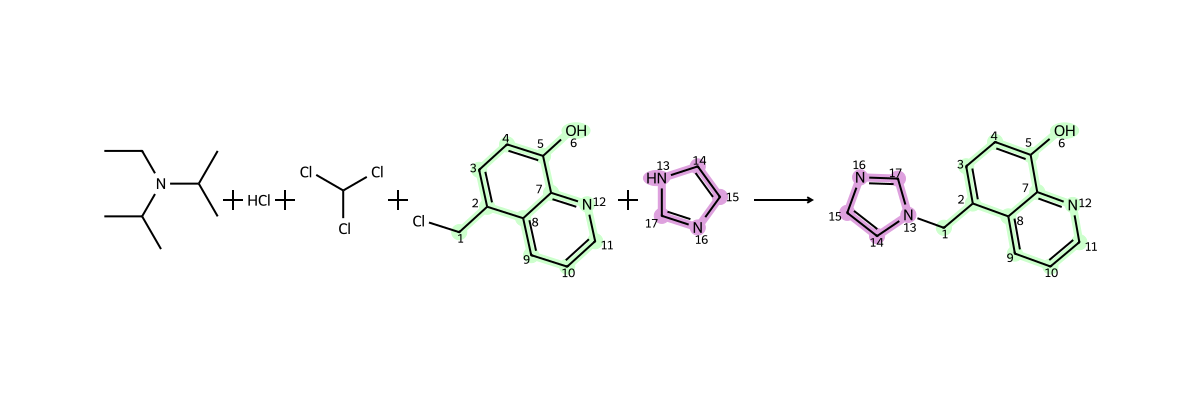
\includegraphics[width=\linewidth]{images/intro_aam_example.png}
  \caption{Example of atom-atom mapping (AAM) for a chemical reaction.}
  \label{fig:aam-example-intro}
\end{figure}

\paragraph{Graph-based approaches.}
Early mapping methods relied on heuristic graph matching.  INDIGO and
related tools use atom-invariant scoring and integer programming to find
optimal correspondences~\cite{Weininger1989}.  While these approaches
are interpretable and fast on small molecules, they do not generalize
well to large or structurally complex reactions.  The benchmarking study of
\citet{Lin2020} systematically evaluated several classical and
hybrid mappers and identified substantial failure rates on USPTO reactions,
motivating the development of data-driven alternatives.

\paragraph{Template-based approaches.}
Another class of AAM approaches assigns atom correspondences by matching
curated reaction SMIRKS or rule-based templates that encode the
mechanistic transformation directly.  NameRxn~\cite{NameRxn} (NextMove
Software) classifies reactions against a large rule base of known
mechanisms and named transformations, establishing atom-level
correspondences as an inherent byproduct of the template match.
Yet even with an exhaustive library of hand-curated templates, coverage
on the USPTO---a corpus that is not particularly chemically diverse---remains only 60--73\%~\cite{Lagerstedt2021},
underscoring the fundamental scalability limits of rule enumeration.
The sheer cost of assembling such rule bases is illustrated by Chematica
(now commercialized as Synthia by MilliporeSigma)~\cite{Szymkuc2016},
whose knowledge base of approximately 115{,}000 expert-coded reaction rules
required over 15~years of continuous curation by PhD-level chemists
to curate.~\cite{Klucznik2018}.

\paragraph{Neural approaches.}
Schwaller et al.~\cite{Schwaller2021} demonstrated that Transformer
encoder models~\cite{Vaswani2017} trained on unlabeled reaction SMILES via MLM
~\cite{Devlin2019} learn atom-mapping as an emergent property of their
attention weights, enabling attention-guided AAM without any labeled
data.  This unsupervised training regime is naturally suited to large
unlabelled reaction corpora such as the USPTO, and achieves strong
overall accuracy, but the MLM objective has no mechanism to explicitly
penalize incorrect correspondences.  In practice, the raw attention
signal is insufficient on its own: introducing a post-hoc neighbour
attention multiplier---which rescales the attention weights of
adjacent atoms before extracting correspondences---improves mapping
correctness by as much as 30\%, with an optimal multiplier of
90 rather than the na\"{i}ve value of 1~\cite{Schwaller2021}.
Correspondences are then extracted via a greedy algorithm which
enforces strict one-to-one assignments; this is appropriate for the
common case but cannot represent reactions in which a single reactant
atom contributes to multiple product atoms.  Residual errors
arise especially for symmetric substrates and reactions where attention
provides insufficient discriminating signal.  Nugmanov
et al.~\cite{Nugmanov2022} (GraphormerMapper) addressed several of these
limitations by replacing SMILES tokenization with a graph-structured
Transformer that carries no positional encodings, making correspondence
prediction invariant to atom and molecule ordering.  Rather than
relying on a single attention head---whose selection is not principled
and can overfit to a particular dataset---GraphormerMapper averages
weights across all heads of the final layer and removes the per-product
normalization step used in RXNMapper, yielding a more stable attention
signal.  Correspondences are then enumerated in a breadth-first-search
order, requiring each newly mapped product atom to be bond-connected to
already-mapped atoms.  Despite these architectural improvements,
GraphormerMapper likewise requires explicit post-hoc engineering for
failure cases: mechanistically incorrect mappings for reaction classes
such as esterification or carbonyl reduction are corrected by a library
of predefined heuristic rules encoded as CGR SMILES and applied via
subgraph isomorphism~\cite{Nugmanov2022}.  The need for a neighbour
attention multiplier in RXNMapper and explicit heuristic correction rules
in GraphormerMapper illustrates a recurring limitation of purely
unsupervised objectives: the training signal alone is insufficient to
guarantee chemically coherent correspondences across all reaction classes,
motivating the integration of curated chemical knowledge alongside learned
representations.

A different strategy was taken by Chen et al.~\cite{Chen2024}
(LocalMapper), who demonstrated that supervised training from
chemist-verified reactions substantially improves AAM accuracy.  Using
a human-in-the-loop active learning framework, LocalMapper trains a
graph neural network on a small set of manually annotated reactions and
iteratively expands coverage by sampling uncertain predictions for
additional human labeling.  Starting from as few as 200 labeled
reactions, LocalMapper achieves state-of-the-art accuracy on the
USPTO-50K benchmark, with confident predictions showing 100\% accuracy
on 3{,}000 randomly sampled reactions~\cite{Chen2024}.  However,
per-reaction manual annotation is inherently expensive: even with
active learning, the labeled set covers only $\sim$1{,}000 reactions
across five labeling rounds, and accuracy on out-of-distribution
reaction classes is bounded by the diversity of the annotated
examples.

\paragraph{This work.}
AgaveChem takes direct inspiration from the observation that supervised
training improves AAM accuracy~\cite{Chen2024}, but replaces
per-reaction annotation with template-level labeling.  The key
insight is that a curated reaction SMIRKS template encodes the atom
correspondence for an entire reaction class: once a template has been
verified, it generates correct ground truth for every reaction in the
dataset that it matches---at no additional annotation cost.  Composing
template matching with an MCS-based partial mapper extends coverage to
reactions without a matching template.  Together, these deterministic
methods produce a labeled training corpus from a filtered subset of the
Lowe USPTO dataset that is orders of magnitude larger than what direct
manual annotation can realistically achieve.  The primary contribution
of this work is a supervised ALBERT-based neural mapper trained on
this labeled corpus.  We show that direct supervision of the attention
alignment objective substantially improves AAM accuracy relative to
purely unsupervised training.

AgaveChem is released as an open-source Python library with four
composable mappers:

\begin{enumerate}[leftmargin=*, label=(\arabic*)]
  \item \textbf{Identical fragment mapper.}  Fragments that appear
        structurally unchanged on both sides of the reaction arrow---counter
        ions, spectator molecules, etc---are detected
        and assigned maps directly, before any other mapper is invoked.
  \item \textbf{MCS mapper.}  Atoms whose local chemical environment is
      unchanged during the reaction are mapped via a modified MCS
      procedure.  Configurable radius parameters control how close to a
      reactive center the mapping extends, yielding conservative partial
      maps that avoid incorrectly assigning atoms near bond-breaking events.
  \item \textbf{Expert template mapper.}  A curated library of reaction
        SMIRKS templates, sourced from ReactionFlash~\cite{ReactionFlash}, Rxn-INSIGHT~\cite{Probst2022},
        and manual curation, is applied to the reaction product.  Mappings from templates
        that generating the expected reactants are retained, breaking ties where necessary using heuristics.
  \item \textbf{Neural mapper.}  An ALBERT transformer trained in two
        phases---unsupervised MLM pre-training followed by multitask
        supervised fine-tuning---that produces complete atom maps via
        attention alignment at inference time.  This is the primary result
        of the paper.
\end{enumerate}

The first three mappers serve a dual role: they generate the labeled
training data for the neural mapper and are themselves released as
independent library components.  The ground truth generation pipeline
is described in \cref{sec:methods}; it produces partial or complete
atom maps for a filtered Lowe USPTO corpus, fully mapping $\sim$60\%
of reactions and covering $\sim$90\% of product atoms.

As a secondary contribution, we release \texttt{rdchiral\_plus}, a
substantially refactored fork of rdchiral~\cite{Coley2019rdchiral}
that is used internally by the template mapper.  It improves speed and fixes a number of 
bugs/issues, including introducing deterministic stereochemistry handling, correcting bond direction
artifacts in conjugated systems, supporting one-pot template application,
and reducing incorrect template roundtrips by 96\% compared to the
original rdchiral and 98\% compared to rdchiral\_cpp.
\Cref{subsec:rdchiral} provides full details.

The paper is organized as follows.  \Cref{sec:related} reviews related
work on atom mapping.  \Cref{sec:methods} describes the AgaveChem
system in full detail.  \Cref{sec:results} presents benchmarks against
existing neural mappers.  \Cref{sec:conclusions} discusses limitations
and directions for future work.

% ---------------------------------------------------------------
\section{Related Work}
\label{sec:related}
% ---------------------------------------------------------------

\todo[inline]{Expand related work section. Key papers to discuss:
  RXNMapper \cite{Schwaller2021}, LocalMapper \cite{Chen2024},
  GraphormerMapper \cite{Nugmanov2022}, Rxn-INSIGHT \cite{Probst2022},
  rdchiral \cite{Coley2019rdchiral}, and the benchmarking study
  \cite{Lin2020}.  Also cover NameRXN/NextMove and classical
  graph-matching approaches.}

% ---------------------------------------------------------------
\section{Methods}
\label{sec:methods}
% ---------------------------------------------------------------

\subsection{System Overview}
\label{subsec:overview}

AgaveChem is structured as a library of four independent mappers
(\cref{fig:overview}) that can be used individually or combined into
a pipeline.  In the default configuration, identical fragments are first
mapped using the identical fragment mapper. Following this, if a mapping 
can be generated using the template mapper, this mapping is returned. If 
not, the reaction proceeds to the neural mapper. Users may also substitute any subset of mappers or
define custom selection strategies.

\begin{figure}[htbp]
  \centering
  \todo[inline]{Insert system overview figure.}
  \caption{Overview of the AgaveChem mapping pipeline.  The four
    mappers (identical fragment, template, MCS, neural) can be used
    independently or composed.  In the ground truth generation phase,
    the first three deterministic mappers are used without the neural
    mapper; at inference time, the neural mapper is used as the
    primary mapper.}
  \label{fig:overview}
\end{figure}

% ---------------------------------------------------------------
\subsection{Dataset Preparation and Ground Truth Generation}
\label{subsec:dataset}
% ---------------------------------------------------------------

\paragraph{Source data.}
We draw from the Lowe USPTO reaction dataset~\cite{Lowe2012}, which
contains \todo{total count} reactions extracted from US patent
literature.  Specifically, we use the subset from XXX.   
We further filter this dataset to remove duplicate reactions, 
reactions that could not be properly canonicalized, reactions that 
fully contain the product as a part of the reactants SMILES. 
We also devise a heuristic to remove reactions that erroneously 
contain a related, but unused chemical as a part of the reaction 
SMILES, typically as a result of a reference to a similar procedure.
An illustrative example is shown in \cref{fig:erroneous-reaction}; 
the following excerpt from the source patent describes the procedure from which the reaction is extracted:

\begin{quote}
\textit{The procedure similar to that of Step 2 of Example 1 was repeated except that 2.82 g of 2-(6'-carbethoxyhexyl)-3-methoxy-4-oxo-2-cyclopenten-1-one and 35 ml of methanol were used instead of 24 g of 2-(6'-carbomethoxyhexyl)-3-methoxy-4-oxo-2-cyclopenten-1-one and isopropanol respectively to provide 2.8 g of 2-(6'-carboethoxyhexyl)-3-methoxy-4-hydroxy-2-cyclopenten-1-one as an oily product.}~\cite{USP3954811}
\end{quote}

\begin{figure}[htbp]
  \centering
  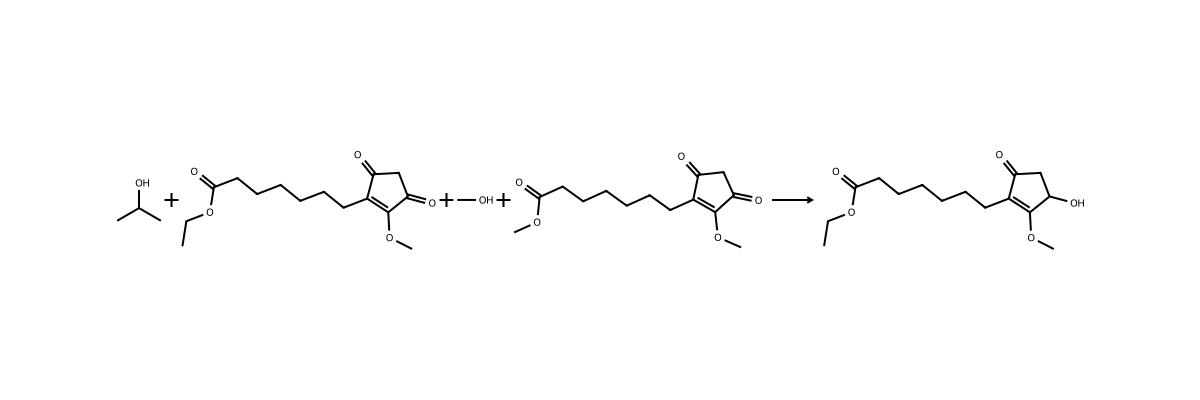
\includegraphics[width=\linewidth]{images/incorrectly_extracted_reaction.png}
  \caption{Example of an erroneously extracted reaction from the USPTO dataset. The reaction SMILES incorrectly includes a related but unused chemical as a reactant, arising from the extraction procedure's reference to a similar prior step in the patent.}
  \label{fig:erroneous-reaction}
\end{figure}

After filtering, approximately
0.97~million reactions remain.  Atom mapping annotations present in
the original dataset are stripped prior to any processing so that the
ground truth is generated entirely by the pipeline described below.

\paragraph{Ground truth generation pipeline.}
The three deterministic mappers are applied sequentially to each
unmapped reaction.  A reaction is considered fully mapped if every
product atom receives a mapping to a unique reactant atom.  Partial
maps (from the MCS mapper) are retained for reactions that are not
fully covered by the template mapper.  \Cref{tab:gt_coverage}
summarizes the coverage achieved at each stage.

\begin{table}[htbp]
  \centering
  \caption{Ground truth coverage at each stage of the deterministic
    mapping pipeline across the $\sim$0.97M filtered USPTO reactions.}
  \label{tab:gt_coverage}
  \begin{tabular}{lcc}
    \toprule
    \textbf{Stage}                 & \textbf{Fully mapped (\%)} & \textbf{Product atoms mapped (\%)} \\
    \midrule
    Identical fragment mapper only & \textit{TBD}               & \textit{TBD}                       \\
    + MCS mapper                   & \textit{TBD}               & \textit{TBD}                       \\
    + Template mapper              & $\sim$60                   & $\sim$90                           \\
    \bottomrule
  \end{tabular}
\end{table}

\subsubsection{Identical Fragment Mapper}
\label{subsubsec:identical_fragment}

The identical fragment mapper handles the simplest class of atom-mapping
decisions: fragments that appear structurally unchanged on both sides of the
reaction arrow.  These include counter-ions, solvent molecules, spectator
reagents, and any other disconnected components whose canonical SMILES is
identical in both the reactant and product.

\paragraph{Algorithm.}
Each reactant and product component is first independently canonicalized with
RDKit~\cite{RDKit}.  A fragment is identified as \emph{identical} if its canonical SMILES
appears in both the reactant component list and the product component list.  For
each such fragment, every atom within the fragment is assigned a unique atom-map number (allocated
from a reserved range starting at 500 to avoid collisions with downstream
mappers), and the fragment is removed from both sides of the reaction before any
other mapper is invoked.  After downstream processing of the reduced reaction,
the pre-mapped identical fragments are reinserted on both sides, yielding a
complete reaction SMILES in which all spectator atoms carry consistent map
numbers.

This design serves a dual purpose.  First, identical spectators are handled
correctly before they can confuse downstream mappers by introducing spurious
reactant--product correspondences.  Second, for reactions in which the only
unmapped components are identical spectators, the mapper provides a complete
map without invoking the more expensive template or MCS procedures.

\subsubsection{MCS Mapper}
\label{subsubsec:mcs}

The MCS mapper assigns atom-map numbers to atoms whose local chemical
environment is preserved across the reaction.  Rather than solving a full
maximum common substructure (MCS) problem---which is NP-hard in general and
scales poorly to multi-fragment reactions---it uses a bond-radius environment
fingerprinting scheme that identifies invariant atoms efficiently and naturally
parameterizes how close to the reactive center the mapping is permitted to
extend.

\begin{figure}[htbp]
  \centering
  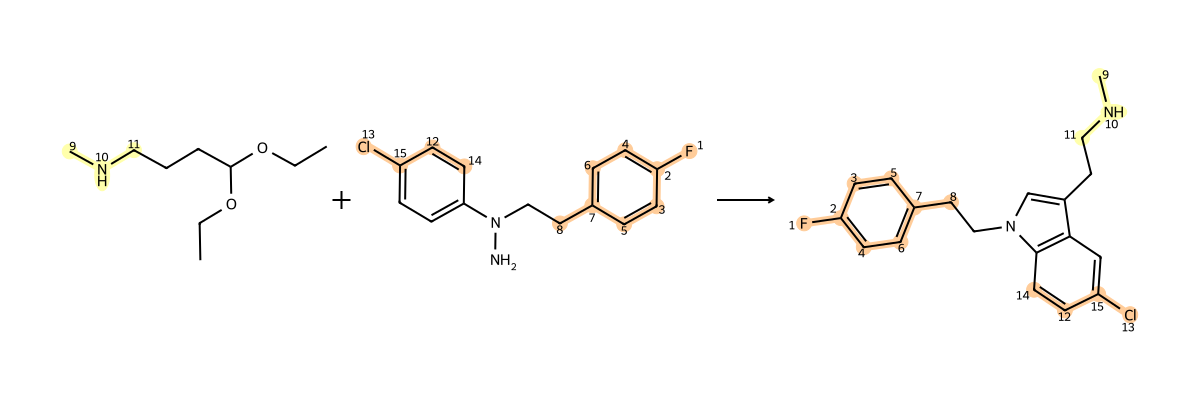
\includegraphics[width=\linewidth]{images/mcs_partial_map.png}
  \caption{Example of partial atom-atom mapping (AAM) for a chemical reaction using the MCS mapper.}
  \label{fig:mcs-partial-map}
\end{figure}

\paragraph{Environment fingerprints.}
For each atom $a$ in a molecule and each integer radius $r$, the mapper
constructs an \emph{environment skeleton}: the canonical ordered list of bonds
lying within $r$ bonds of $a$, extracted via RDKit's
\texttt{FindAtomEnvironmentOfRadiusN} and sorted by RDKit canonical atom ranks.
From this skeleton a hashable, index-free \emph{fingerprint} is computed by
encoding, for each bond in the skeleton, the BFS distance from $a$ to each bond
endpoint together with the chemical properties of those endpoints (atomic
number, formal charge, aromaticity, ring membership, total hydrogen count, and
degree) and the bond itself (bond order, stereo).  Two environments are
considered identical if and only if their fingerprints match.  The fingerprint
also incorporates atom-map numbers as they are assigned, so environments containing
already-mapped atoms acquire a distinct signature that anchors subsequent
matching.

Prior to fingerprint computation, each molecule is normalized by neutralizing
formal charges and canonicalizing its tautomeric form via RDKit's
\texttt{Uncharger} and \texttt{TautomerEnumerator}.  This prevents charge
variants and tautomers from generating spurious fingerprint mismatches for
otherwise equivalent atoms.

\paragraph{Radius search.}
Fingerprints are built incrementally, starting from a minimum radius
(default 1) and increasing until a unique reactant--product atom fingerprint
match is found or all matches disappear.  Atoms whose environment has no
cross-side match at a given radius are pruned and skipped at all subsequent
radii as an optimization.  The largest radius at which at least
one match was found is used as the \emph{final radius} for the subsequent
mapping phase.

\paragraph{Anchor-extend assignment.}
Once the final radius is determined, atom-map numbers are assigned via an
\emph{anchor-extend} strategy alternating between two phases:

\begin{enumerate}[leftmargin=*, label=(\arabic*)]
  \item \textbf{Extend phase.}  Scanning from the highest radius down to
        radius~1, the mapper identifies reactant--product fingerprint pairs that
        contain at least one already-mapped atom (\emph{anchored} matches).
        Because the fingerprint includes existing map numbers, an anchored match
        is unambiguous: the matched atom is adjacent to a confirmed
        correspondence and can be safely propagated.  The full sweep repeats
        until no further anchored matches remain.
  \item \textbf{New-anchor phase.}  A single unanchored match is selected at
        the highest available radius (at or above
        \texttt{min\_radius\_to\_anchor\_new\_mapping}, default~3) and assigned,
        then control returns to the extend phase.
\end{enumerate}

This ordering ensures that each anchor is fully propagated before a new
independent anchor is introduced, preventing inconsistent mapping chains.  A
candidate assignment is additionally rejected if the product atom has an
already-mapped neighbor that was sourced from a different reactant molecule,
enforcing structural adjacency consistency.

\paragraph{Conservative partial mapping.}
The \texttt{min\_radius\_to\_anchor\_new\_mapping} and \texttt{min\_radius} 
parameters controls conservatism of the partial map.  At low radii, local environments are too generic to
uniquely distinguish atoms that are unchanged from those involved in bond-making
or bond-breaking events.  By requiring new unanchored matches to carry at least
radius~3 of local context, the mapper abstains from assigning atoms in
ambiguous positions.  The result is a conservative \emph{partial} map: atoms
well removed from the reaction site receive confident assignments, while atoms
near the reactive center are left unmapped for the neural mapper to resolve.

\subsubsection{Expert Template Mapper}
\label{subsubsec:template}

The template mapper applies a curated library of reaction SMIRKS to each
reaction product and accepts a mapping when the virtual reactants generated by
the template match the actual reactants after canonicalization.  Because the
template encodes the mechanistic atom correspondence explicitly, every accepted
map correctly captures bond-breaking and bond-forming events---not merely the
invariant substructure.  This makes template-produced maps the highest-quality
ground truth in the pipeline.

\begin{figure}[htbp]
  \centering
  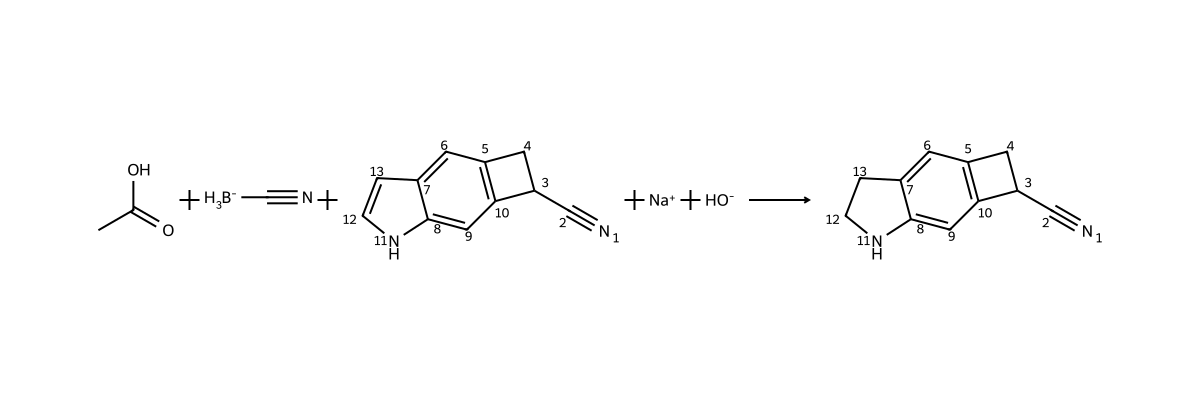
\includegraphics[width=\linewidth]{images/template_map.png}
  \caption{Example of atom-atom mapping (AAM) for a chemical reaction using the template mapper, in this case
  using the template "Gribble Indole Reduction; Indole reduction to indoline (NaBH3CN/TFA)".}
  \label{fig:template-map}
\end{figure}

\paragraph{Template library.}
Templates were assembled from three sources: (1) the Rxn-INSIGHT library of
named reaction patterns~\cite{Probst2022}; (2) templates extracted from the
ReactionFlash iOS application; and (3) a set of nucleophilic substitution
templates generated programmatically.  All templates were reviewed and, where
necessary, corrected by hand.  Each parent SMIRKS is expanded into one or more
\emph{child} SMIRKS that capture specific substitution patterns or
stereo-variants of the parent; templates are applied at the child level.  Each
template carries an optional two-level priority tuple
\texttt{(priority\_class, priority)} used for tie-breaking when multiple
templates produce different maps for a single reaction.  Template application is performed using
\texttt{rdchiral\_plus} (\cref{subsec:rdchiral}).

\begin{lstlisting}[language=json, caption={Example template reaction record.}, label={lst:template-record}, basicstyle=\footnotesize\ttfamily, float=htbp]
{
  "class_id": 5,
  "name": "Prilezhaev Epoxidation; mCPBA epoxidation of alkene",
  "priority": {
      "priority_class": 3,
      "priority": 5
  },
  "smirks": "[C:1]=[C:2].[O;H1:3]-OC(=O)c1cccc(Cl)c1>>[C:1]1-[O:3]-[C:2]1",
  "subclass_id": 1,
  "subsubclass_id": null,
  "superclass_id": 10,
  "rxno_classification": [
      {
          "rxno_id": "RXNO:0000405"
      }
  ]
}
\end{lstlisting}

\paragraph{MCS pre-pass.}
Before any template is applied, the MCS mapper is run on the input reaction to
produce a partial map.  Connected components of product atoms that the MCS
mapper could not assign---atoms near the reactive center whose local environment
is not uniquely shared with a reactant atom---are identified as \emph{unmapped
islands}.  Template application is then restricted to templates whose product
SMARTS overlaps with an atom in at least one unmapped island.  This focuses the template
search on the reaction center and avoids wasting time on templates that would
only remap atoms already conservatively assigned by the MCS mapper.

\paragraph{Two-tier template screening.}
For each template, candidate viability is assessed in two stages before the
full rdchiral application is invoked:

\begin{enumerate}[leftmargin=*, label=(\arabic*)]
  \item \textbf{Fingerprint pre-screen.}  RDKit \texttt{PatternFingerprint}
        vectors are pre-computed for every template fragment and for every
        product and reactant molecule.  A template is discarded immediately if
        any of its required product or reactant bits are absent from the
        corresponding molecular fingerprints (\texttt{AllProbeBitsMatch}).
  \item \textbf{Substructure pre-screen.}  For templates that pass the
        fingerprint check, each template fragment must have at least one
        substructure match in the product molecules and in the
        reactant molecules.  Additionally, the product
        check is further tightened: a template fragment is accepted only if its
        substructure match has at least partial overlap with an unmapped island.
\end{enumerate}

Only templates passing both screens are forwarded to full rdchiral application.

\paragraph{Template application and outcome validation.}
Templates passing both screens are applied to the product using
\texttt{rdchiralRun}, which returns virtual reactant SMILES together with the
atom map indices of the affected atoms.  Each outcome is then validated:

\begin{enumerate}[leftmargin=*, label=(\arabic*)]
  \item \textbf{Fragment matching.}  The virtual reactant fragments are
        compared against the actual reactants (and their tautomers, enumerated
        once per reaction).  A fragment is considered matched if its canonical
        SMILES---with atom map numbers stripped---appears in the tautomer set
        of any actual reactant.
  \item \textbf{Wildcard fragment resolution.}  Templates with wildcard atoms
        (\texttt{*}) produce fragments whose canonical form does not directly
        match an actual reactant.  For these, the mapper attempts to transfer
        the template's atom-map numbers to the actual reactant via substructure
        matching.  The transfer is accepted only when the match is unique or
        when all matches are symmetry-equivalent (i.e.\ the molecule is
        symmetric with respect to the query), preventing ambiguous assignments.
  \item \textbf{Spectator reconciliation.}  Any actual reactant component not
        present in the template outcome is reattached as an unmapped spectator
        so that the final reaction SMILES accounts for all input fragments.
\end{enumerate}

An outcome is rejected if any fragment cannot be matched or resolved.

\paragraph{Outcome selection.}
Valid outcomes are canonicalized and deduplicated.  Each candidate is
cross-checked by stripping its atom-map numbers and verifying that the
resulting reaction SMILES is identical to the canonicalized input reaction,
ensuring the template did not introduce or remove atoms.  If
multiple distinct valid outcomes remain after deduplication, the preferred
mapping is selected first by template priority class, then by intra-class
priority, and finally---when no explicit priority is set---by the total atom
count of the matching template (more structurally specific templates are
preferred).

% ---------------------------------------------------------------
\subsection{Neural Mapper Architecture}
\label{subsec:neural_arch}
% ---------------------------------------------------------------

The neural mapper follows the same general architecture as
RXNMapper~\cite{Schwaller2021}: an ALBERT transformer encoder whose
attention weights in a designated head and layer are used to produce
atom-to-atom correspondences.  The model uses the same ALBERT
configuration as RXNMapper (hidden size 256, 12 layers, 8 attention
heads, intermediate size 512, embedding size 128), but with a
custom vocabulary of size 1024 tokens designed specifically for
reaction SMILES.  Reactions are tokenized at the atom level using a
custom tokenizer that treats each SMILES atom token (including bracket
atoms and isotope specifications) as a single unit, preserving bond,
ring closure, and branch tokens as separate tokens.

For supervised training, we augment the base ALBERT model with a
dedicated attention alignment head.  The alignment head extracts the
raw attention logits from a specific layer and head(s) identified during
the unsupervised pre-training phase, applies a final linear projection,
and computes a KL-divergence loss against the ground truth alignment
matrix.  Unmapped atoms that are confidently do not participate in the reaction
 and non-atom tokens (bonds, parentheses,
ring-closure digits) are directed to a special ``sink'' token, making
the loss well-defined even for partially labeled reactions.  Symmetric
atoms---those that belong to symmetry-equivalent groups as determined
by RDKit's canonical ranking---receive smoothed targets that distribute
probability uniformly over the symmetric group, preventing the model
from being penalized for correct but arbitrarily labeled assignments.

\begin{figure}[htbp]
  \centering
  \todo[inline]{Insert model architecture figure: ALBERT encoder,
    attention alignment head, supervised loss.}
  \caption{AgaveChem neural mapper architecture.  A custom attention
    alignment head extracts logits from a designated attention head and
    computes a cross-entropy loss against the ground truth alignment
    matrix.  Unmapped atoms are directed to a sink token.  Symmetric
    atoms receive smoothed targets.}
  \label{fig:arch}
\end{figure}

% ---------------------------------------------------------------
\subsection{Training Procedure}
\label{subsec:training}
% ---------------------------------------------------------------

Training proceeds in two phases.

\subsubsection{Phase 1: Unsupervised MLM Pre-training}
\label{subsubsec:pretrain}

In the first phase, the base ALBERT model is trained on the full
corpus of filtered USPTO reactions using masked language modeling.
We adopt a graph-aware span masking strategy in place of the standard
independent token masking used by RXNMapper.  Rather than selecting
individual tokens uniformly at random, the masking procedure selects
contiguous neighborhoods of atoms on the molecular graph, using BFS
from a randomly chosen seed atom with a stochastic span size drawn
from a weighted distribution over $\{1, 2, 3, 4, 5\}$ atoms.  Only
atom tokens are eligible for masking; structural tokens (bond symbols,
parentheses, ring-closure digits) are never masked.  For each masked
atom, the replacement follows a modified 70/20/10 strategy: 70\% of
the time the token is replaced with \texttt{[MASK]}, 20\% of the time
it is replaced with a chemically plausible alternative, and 10\% of the time the
original token is retained.  Random SMILES augmentation is applied
at each epoch: with 5\% probability the canonical form is used;
otherwise, a random SMILES enumeration of the reaction is sampled,
with a 10\% probability of also randomizing the tautomer.

The model is trained with AdamW with a learning rate of
$2 \times 10^{-4}$, weight decay $10^{-3}$, linear warmup over
10,000 steps, and gradient clipping at 1.0.  The masking probability
is 15\% in this phase.

\subsubsection{Phase 2: Multitask Supervised Fine-tuning}
\label{subsubsec:finetune}

In the second phase, training continues on all reactions for which
ground truth atom maps are available---both fully and partially mapped
by the deterministic pipeline.  Fully mapped reactions ($\sim$60\% of
the labeled corpus) contribute supervision over all product atoms;
partially mapped reactions contribute supervision over only the subset
of atoms that received a ground truth assignment.  The training
objective is a weighted combination of the MLM loss and the supervised
attention alignment loss:
\begin{equation}
  \mathcal{L} = \lambda_{\mathrm{MLM}} \cdot \mathcal{L}_{\mathrm{MLM}}
  + \lambda_{\mathrm{align}} \cdot \mathcal{L}_{\mathrm{align}},
  \label{eq:loss}
\end{equation}
where $\mathcal{L}_{\mathrm{align}}$ is the per-atom KL divergence
between the predicted attention distribution and the ground truth
alignment matrix, computed only over atoms for which a ground truth
mapping is available.  Continuing the MLM objective prevents
catastrophic forgetting and encourages the model to maintain the
chemical representation learned in Phase~1.  The same masking probability
and weighted distribution over span sizes is used as in Phase~1.

\todo[inline]{Report final $\lambda$ values and other hyperparameters
  after ablation experiments.}

% ---------------------------------------------------------------
\subsection{Inference}
\label{subsec:inference}
% ---------------------------------------------------------------

\paragraph{Input preparation.}
A reaction SMILES of the form \texttt{reactants>>products} is tokenized
using the custom SMILES tokenizer described in \cref{subsec:pretraining}.
The reaction arrow token \texttt{>>} is retained in the sequence and acts
as a structural boundary between the two sides of the reaction.
During tokenization, each position is classified as either a heavy-atom token
(annotated with its element identity) or a non-atom token (bond symbols, ring
closures, parentheses, brackets, etc.); this classification is used in the
subsequent masking step.

\paragraph{Attention extraction.}
The tokenized sequence is passed through the model in a single forward pass.
For the supervised \texttt{AlbertWithAttentionAlignment} model, a dedicated
output head produces a full-sequence attention matrix of shape
$S \times S$ directly.
For the unsupervised ALBERT baseline, the raw attention weights from a
designated layer and head are extracted via
the standard \texttt{output\_attentions} interface.
In both cases the resulting matrix is log-transformed before downstream
processing.

\paragraph{Attention masking.}
The log-attention matrix is masked to enforce chemical validity constraints.
Self-side attention (reactant-to-reactant and product-to-product) is
suppressed by setting the corresponding logits to $-10^6$, and attention
to or from non-atom tokens is likewise suppressed, with the exception 
of reactant atom's attention to the sink token.
Attention between tokens of \emph{different element types} is
also masked to $-10^6$, constraining proposed correspondences to
same-element atom pairs.
The masked logit matrix is then row-normalised via softmax, allocating all
probability mass within each row to the remaining cross-reaction,
element-matched positions.

\paragraph{Cross-attention alignment and symmetry correction.}
The masked probability matrix is sliced into two cross-attention sub-matrices:
$\mathbf{A}^{P \to R}$ (product tokens attending to reactant tokens, shape
$n_{\text{prod}} \times n_{\text{react}}$) and $\mathbf{A}^{R \to P}$
(reactant tokens attending to product tokens, transposed to the same
orientation).  Both matrices are further reduced to heavy-atom positions
only by removing the rows and columns that correspond to non-atom tokens.
To prevent probability mass from being artificially split among
topologically equivalent atoms (e.g.\ the ortho positions of an
unsubstituted arene), the columns (reactant symmetry) or rows (product
symmetry) belonging to each symmetric group are summed before decoding;
topological equivalence is determined by RDKit canonical ranks computed
over the combined reactant or product graph.

\paragraph{Greedy one-to-one assignment.}
The two atom-level cross-attention sub-matrices are averaged element-wise
to form a single scoring matrix.  Map numbers are then assigned by a greedy
globally-aware procedure: at each iteration, the global maximum of the
current scoring matrix is located; the corresponding product and reactant
atoms receive the next available map number; and the entire row and column
of that entry are zeroed by default to enforce a bijective correspondence.
After each assignment, the attention scores of unassigned neighbors of the
just-mapped pair are boosted by a multiplier (default $\times 10$) to
encourage locally consistent mappings, with an additional multiplier
(default $\times 10$) when a candidate neighbor pair shares the same
element encoding.
The overall reaction-level confidence score is the product of the
per-atom attention probabilities at each selected position, taken from the
symmetry-corrected scoring matrix before any neighborhood boosting is
applied.

\paragraph{Batched inference.}
To amortise the cost of transformer inference, reactions are processed in
configurable batches (default 32).  Within each batch, all reaction SMILES
strings are tokenized and padded to a common maximum length (default 512
tokens) to form a single dense input tensor; invalid reactions are skipped
before batching and receive an empty result.  One forward pass of the model
then produces the full attention tensor for all sequences simultaneously.
Because all sequences in a batch are padded to the same length, each
resulting attention matrix is trimmed to the reaction's true (non-padding)
length by counting the non-zero entries in the corresponding
\texttt{attention\_mask} row before any downstream processing.  Atom-map
assignment and confidence scoring are subsequently performed per reaction
on the CPU from the pre-computed (and padding-stripped) attention matrices,
so that GPU time is concentrated entirely in the batched forward pass.

% ---------------------------------------------------------------
\subsection{\texttt{rdchiral\_plus}}
\label{subsec:rdchiral}
% ---------------------------------------------------------------

The expert template mapper relies on fast, accurate and reproducible template
application.  The original rdchiral library~\cite{Coley2019rdchiral},
while widely used, contains several classes of errors that affect both
template extraction and application.  We developed
\texttt{rdchiral\_plus}, a fork of rdchiral with the following
improvements.

\paragraph{Template application.}
\begin{itemize}[leftmargin=*]
  \item \emph{Conjugated system bond direction correction.}  Corrupted
        single-bond directions (\texttt{ENDUPRIGHT}, \texttt{ENDDOWNRIGHT})
        that arise in conjugated systems are detected and corrected.
  \item \emph{Broader stereochemistry handling.}  Tetrahedral centers
        with lone pairs are now handled correctly.
  \item \emph{One-pot reactions.}  Templates defining multiple
        transformations on the same product are initialized with
        parentheses, enabling correct handling of multi-site reactions.
  \item \emph{Recursive template application.}  Templates can be
        applied recursively with a configurable maximum depth, which is
        necessary for symmetric reactions or reactions occurring at
        multiple sites.
\end{itemize}

\paragraph{Template extraction.}
\begin{itemize}[leftmargin=*]
  \item \emph{Configurable radius.}  Template extraction supports a
        configurable radius and special group handling.
  \item \emph{Deterministic extraction.}  The random shuffle-based
        tetrahedral correction loop in the original implementation is
        replaced with a deterministic permutation parity calculation,
        eliminating rare hangs and non-reproducible outputs.
  \item \emph{Stereochemistry tracking.}  Inversion of tetrahedral
        centers is now counted as a changed atom and included in extracted
        templates.
  \item \emph{Spectator tracking.}  Spectator molecules are included
        in extracted template dictionaries.
\end{itemize}

\paragraph{Consistency with rdchiral.}
Roundtrip consistency---extracting a template from a mapped reaction
SMILES and re-applying it to the product to recover the expected
reactants---is used to quantify correctness.  \texttt{rdchiral\_plus}
reduces incorrect roundtrips by 96\% compared to rdchiral and by 98\%
compared to rdchiral\_cpp.  \Cref{tab:rdchiral} summarizes the
comparison.

\begin{table}[htbp]
  \centering
  \caption{Roundtrip consistency of template extraction and application
    across the three rdchiral variants.  A roundtrip is considered
    correct if re-applying the extracted template to the product
    recovers the expected reactant SMILES.}
  \label{tab:rdchiral}
  \begin{tabular}{lcc}
    \toprule
    \textbf{Library} & \textbf{Incorrect roundtrips (\%)} & \textbf{Reduction vs.\ rdchiral\_plus} \\
    \midrule
    rdchiral         & 1.59\%                          & $-$96\%                                \\
    rdchiral\_cpp    & 2.64\%                          & $-$98\%                                \\
    rdchiral\_plus   & 0.06\%                          & ---                                    \\
    \bottomrule
  \end{tabular}
\end{table}

% ---------------------------------------------------------------
\section{Results and Discussion}
\label{sec:results}
% ---------------------------------------------------------------

We evaluate AgaveChem against three established neural
mappers---RXNMapper~\cite{Schwaller2021}, LocalMapper~\cite{Chen2024},
and GraphormerMapper~\cite{Nugmanov2022}---using the benchmark protocol
and evaluation sets described in~\cite{Lin2020,Jaworski2019}, employing
held-out reactions drawn from the USPTO and graph isomorphism
to determine whether a proposed mapping is equivalent to the reference.
All reactions included in any evaluation set were withheld from
AgaveChem's training corpus prior to training.  We report two primary
metrics: \emph{exact match accuracy}, defined as the fraction of
reactions for which every product atom is correctly mapped to its
reference counterpart, and \emph{per-atom accuracy}, defined as the
fraction of individual product atoms across all test reactions that
receive the correct mapping.  Exact match is the more stringent
criterion; per-atom accuracy better characterizes performance on
partial or near-correct mappings and is informative for reactions
where the model assigns only a small number of atoms incorrectly.

% ---------------------------------------------------------------
\subsection{Benchmark Datasets and Evaluation Metrics}
\label{subsec:benchmark}
% ---------------------------------------------------------------

\todo[inline]{Describe the benchmark dataset(s) in detail: source,
  size, reaction types covered, split strategy.  Reference the
  benchmarking study of Jaworski et al.\ and any additional evaluation
  sets used.}

\paragraph{Evaluation metric.}
A predicted mapping is compared against a reference mapping using a
graph-isomorphism test rather than a literal string comparison.  Each
mapped reaction SMILES is first converted into an undirected bipartite
graph in which nodes represent heavy atoms and edges represent either
intramolecular bonds or atom-mapping correspondences.  Every node
carries the full atom environment---atomic number, formal charge,
aromaticity, ring membership, total hydrogen count, degree, and CIP
chirality tag---and every bond edge carries its bond order and stereo
descriptor.  Two mappings are declared equivalent if and only if a
graph isomorphism exists that simultaneously matches all node and edge
attributes.  This approach correctly identifies mappings that are
alphabetically different but chemically identical (e.g.\ when map
numbers are permuted but all correspondences are preserved), and it
properly penalizes mappings that differ only in stereochemistry.

\paragraph{Tautomer equivalence.}
A strict string- or even graph-level comparison can incorrectly
penalise a correct mapping when the reaction involves a tautomerisable
species.  Consider the N-alkylation of imidazole illustrated in
\cref{fig:aam-example-intro}: a terminal chloroalkyl reacts at the
NH nitrogen of imidazole, but the two tautomeric forms of the free
base exchange the NH proton between the two ring nitrogens.  As drawn,
the attacked nitrogen carries the NH, yet a mapper that assigns the
bond-forming event to the other ring nitrogen produces an equally
valid description of the same reaction.  To handle such cases,
when tautomer-aware comparison is enabled, all tautomeric forms of
each reactant and product fragment in the predicted reaction are
enumerated (using RDKit's \texttt{TautomerEnumerator}), and the
isomorphism test is performed against the full Cartesian product of
tautomeric combinations.  The reference mapping is held fixed; a
prediction is accepted if it matches any tautomeric variant of the
reference.

\paragraph{Resonance equivalence.}
A complementary correction handles mappings that differ only in the
assignment of atom-map numbers between resonance-equivalent atoms.
For a small set of structural motifs---nitro groups
($\mathrm{O{=}N^{+}O^{-}}$), carboxylates ($\mathrm{O{=}CO^{-}}$),
carboxylic acids ($\mathrm{O{=}COH}$), and sulfonates
($\mathrm{O{=}S({=}O)O^{-}}$)---atom-map numbers may legitimately
be exchanged between the two equivalent oxygen atoms without changing
the chemistry of the mapping.  When resonance-swap comparison is
enabled, all $2^n$ combinations of such swaps (for $n$ candidate
pairs) are enumerated for the predicted mapping, and the prediction is
accepted if any combination is isomorphic to the reference.

% ---------------------------------------------------------------
\subsection{Comparison with Existing Neural Mappers}
\label{subsec:comparison}
% ---------------------------------------------------------------

\begin{table}[htbp]
  \centering
  \caption{Atom mapping accuracy on the benchmark test set.
    Exact match: fraction of reactions with all atoms correctly mapped.
    Per-atom: fraction of individual product atoms correctly mapped.
    All AgaveChem results use the neural mapper.}
  \label{tab:main_results}
  \begin{tabular}{lcc}
    \toprule
    \textbf{Method}                      & \textbf{Exact match (\%)} & \textbf{Per-atom (\%)} \\
    \midrule
    RXNMapper~\cite{Schwaller2021}       & \textit{TBD}              & \textit{TBD}           \\
    LocalMapper~\cite{Chen2024}          & \textit{TBD}              & \textit{TBD}           \\
    GraphormerMapper~\cite{Nugmanov2022} & \textit{TBD}              & \textit{TBD}           \\
    \midrule
    AgaveChem (neural)                   & \textbf{\textit{TBD}}     & \textbf{\textit{TBD}}  \\
    AgaveChem (combined)                 & \textbf{\textit{TBD}}     & \textbf{\textit{TBD}}  \\
    \bottomrule
  \end{tabular}
\end{table}

\todo[inline]{Write the body of this subsection once benchmark numbers
  are available.  Key points: (1) AgaveChem outperforms LocalMapper and
  substantially outperforms RXNMapper; (2) characterize where remaining
  errors occur; (3) include qualitative examples.}

\todo[inline]{Discussion of USPTO-50k and 3k}

\todo[inline]{Discussion of Golden dataset errors}

\todo[inline]{Discussion of USPTO-50k and USPTO-3k}

% ---------------------------------------------------------------
\subsection{Prediction Confidence}
\label{subsec:prediction_confidence}
% ---------------------------------------------------------------

The neural mapper produces a scalar confidence score for each predicted
mapping, derived from the attention alignment logits.  To evaluate the
discriminative quality of this score we treat the task as binary
classification---a mapping is labelled \emph{correct} if it matches the
deterministic ground truth and \emph{incorrect} otherwise---and assess
the model's ability to distinguish the two classes on a held-out test
set of \todo{N} reactions.

\begin{table}[htbp]
  \centering
  \caption{Binary classification performance of the neural mapper
    confidence score on the held-out test set.}
  \label{tab:confidence_metrics}
  \begin{tabular}{lc}
    \toprule
    \textbf{Metric} & \textbf{Value} \\
    \midrule
    Accuracy  & 0.767 \\
    Precision & 0.972 \\
    Recall    & 0.765 \\
    F1-Score  & 0.857 \\
    AUC       & 0.842 \\
    \bottomrule
  \end{tabular}
\end{table}

The confusion matrix on the test set contains
$\mathrm{TP} = 1{,}224$, $\mathrm{TN} = 123$, $\mathrm{FP} = 35$, and
$\mathrm{FN} = 375$ predictions.  The very high precision (0.972) with
relatively lower recall (0.765) indicates that when the confidence score
flags a mapping as correct, it almost never makes a false positive
error; however, a meaningful fraction of genuinely correct mappings
receive a low confidence score and are consequently under-counted.
The AUC of 0.842 confirms that the score provides reliable rank
ordering across the full confidence range.

\todo[inline]{Expand: describe the confidence threshold used, the
  class imbalance in the test set, and how the score is used at
  inference time (e.g.\ fallback to MCS mapper below a threshold).}

% ---------------------------------------------------------------
\subsection{Template Mapper Performance}
\label{subsec:template_perf}
% ---------------------------------------------------------------

\todo[inline]{Report template mapper performance on named reactions:
  exact match rate for template-covered reactions, coverage across
  reaction classes, comparison to rule-based mappers.}

% ---------------------------------------------------------------
\subsection{Ground Truth Quality Analysis}
\label{subsec:gt_quality}
% ---------------------------------------------------------------

\todo[inline]{Analyze the quality of the generated ground truth:
  sample a subset of fully mapped reactions and verify against manual
  annotation or alternative references; characterize which reaction
  classes the deterministic pipeline fails to map.}

% ---------------------------------------------------------------
\section{Conclusions}
\label{sec:conclusions}
% ---------------------------------------------------------------

We have presented AgaveChem, an open-source atom-to-atom mapping
library that combines deterministic expert knowledge with supervised
neural learning.  The library provides four composable mappers---identical
fragment, expert template, MCS, and neural---each targeting a different
subset of the atom mapping problem and suited to different downstream
use cases.

The central contribution is the supervised training strategy for the
neural mapper.  Rather than relying solely on unsupervised MLM, we use the
deterministic mappers to generate labeled ground truth from a filtered
Lowe USPTO corpus, then apply this data to directly supervise the
attention alignment objective during fine-tuning.  The result is a
model that retains the broad reaction coverage of attention-based
neural mappers while substantially reducing the class of errors that
arise from inferring atomic correspondence without explicit supervision.  
The deterministic mappers that produce the
training labels are themselves useful tools, covering $\sim$60\% of
reactions fully and $\sim$90\% of product atoms across the USPTO corpus.

The expert template mapper is notable as a standalone tool.  For
reactions that match a known named reaction pattern, it produces maps
that are by construction mechanistically consistent, making it
particularly well-suited for downstream applications besides atom-to-atom mapping,
 such as reaction classification.

As a byproduct of this work, we release \texttt{rdchiral\_plus}, a
substantially improved fork of rdchiral.  The 96\% reduction in
incorrect template roundtrips directly improves the quality of the
generated ground truth and, through it, the quality of the trained
neural model.

\paragraph{Limitations and future work.}
The ground truth generation pipeline produces only partial maps for
roughly 40\% of training reactions, leaving the neural model to
generalize over reaction types that are underrepresented in the labeled
data.  While the model already outperforms existing baselines,
performance on unusual reaction classes and highly symmetric substrates
remains an area for improvement.

The pipeline is well-suited to incremental improvement: expanding the expert
template library---particularly for less common named reactions and multi-step
transformations---directly increases the fraction of fully labeled training
reactions at no additional per-reaction annotation cost.  More broadly, any
deterministic method that can precisely establish product atom
provenance---additional template sources, curated mechanistic rules, or
reaction-class-specific substructure procedures---slots naturally into the same
pipeline.  Likewise, any method that can precisely determine which reactant atoms
do \emph{not} correspond to any product atoms, for example, by comparing stoichiometric ratios of reactants and products, may
also be easily integrated into the pipeline.  As always, training on a larger, higher-quality,
and more chemically diverse corpus would be expected to improve
generalization, especially for underrepresented or complex reaction classes.

The labeled ground truth produced by the deterministic pipeline is
architecture-agnostic.  While the current neural mapper uses an ALBERT-based
SMILES encoder, the same supervision signal could be applied to graph neural
network architectures, alternative transformer models, or other sequence
encoders that operate on reaction SMILES.  No systematic hyperparameter search
or architecture ablation was conducted in this work; exploring these dimensions
represents a natural direction for future investigation.

\todo[inline]{Further improvements to AgaveChem app - reranking, scoring, extensible mapping.}

% ---------------------------------------------------------------
\section*{Data and Software Availability}

AgaveChem is released as an open-source Python library under the MIT
license at \url{https://github.com/denovochem/agave_chem}.
\texttt{rdchiral\_plus} is available at
\url{https://github.com/denovochem/rdchiral_plus}.
Remapped versions of the USPTO-50K and USPTO-Full benchmark datasets,
produced using the AgaveChem deterministic mapping pipeline, are available at
\url{https://PLACEHOLDER\_URL}.
\todo[inline]{Add data availability statement for the training set
  and benchmark reactions.}

% ---------------------------------------------------------------
\bibliographystyle{unsrtnat}
\bibliography{references}

% ---------------------------------------------------------------
% Placeholder bibliography (replace with references.bib)
% ---------------------------------------------------------------
\begin{thebibliography}{99}

  \bibitem{Schwaller2021}
  Schwaller, P.; Hoover, B.; Reymond, J.-L.; Strobelt, H.; Laino, T.
  Extraction of organic chemistry grammar from unsupervised learning of
  chemical reactions.
  \emph{Science Advances} \textbf{2021}, \emph{7}(15), eabe4166.

  \bibitem{Chen2024}
  Chen, S.; An, S.; Babazade, R.; Jung, Y.
  Precise atom-to-atom mapping for organic reactions via human-in-the-loop
  machine learning.
  \emph{Nat.\ Commun.} \textbf{2024}, \emph{15}, 2250.

  \bibitem{Nugmanov2022}
  Nugmanov, R.; Dyubankova, N.; Gedich, A.; Wegner, J.~K.
  Bidirectional Graphormer for Reactivity Understanding: Neural Network
  Trained to Reaction Atom-to-Atom Mapping Task.
  \emph{ChemRxiv} \textbf{2022}. \url{https://doi.org/10.26434/chemrxiv-2022-bn5nt}

  \bibitem{Probst2022}
  \todo{Rxn-INSIGHT full citation (Probst et al.).}

  \bibitem{Coley2019rdchiral}
  Coley, C.~W.; Green, W.~H.; Jensen, K.~F.
  RDChiral: An RDKit Wrapper for Handling Stereochemistry in
  Retrosynthetic Template Extraction and Application.
  \emph{J.\ Chem.\ Inf.\ Model.} \textbf{2019}, \emph{59}(6), 2529--2537.

  \bibitem{Coley2019}
  Coley, C.~W.; Thomas, D.~A.; Lummiss, J.~A.~M.; Jaworski, J.~N.;
  Breen, C.~P.; Schultz, V.; Hart, T.; Fishman, J.~S.; Rogers, L.;
  Gao, H.; Hicklin, R.~W.; Plehiers, P.~P.; Byington, J.; Pierson, J.~S.;
  Burns, J.~W.; Dixon, A.~G.; Hwang, A.; Gonzalez-Hernandez, M.;
  Couillard, S.~A.~E.; Hayashi, T.; Green, W.~H.; Jensen, K.~F.
  A robotic platform for flow synthesis of organic compounds informed by
  AI planning.
  \emph{Science} \textbf{2019}, \emph{365}(6453), eaax1566.

  \bibitem{Lin2020}
  Lin, A.; Dyubankova, N.; Madzhidov, T.~I.; Nugmanov, R.; Rakhimbekova, A.;
  Ibragimova, Z.; Akhmetshin, T.; Gimadiev, T.~R.; Suleymanov, R.;
  Verhoeven, J.; Wegner, J.~K.; Ceulemans, H.; Varnek, A.
  Atom-to-Atom Mapping: A Benchmarking Study of Popular Mapping Algorithms
  and Consensus Strategies.
  \emph{ChemRxiv} \textbf{2020}. \url{https://doi.org/10.26434/chemrxiv.13012679.v1}

  \bibitem{Lan2020}
  Lan, Z.; Chen, M.; Goodman, S.; Gimpel, K.; Sharma, P.; Soricut, R.
  ALBERT: A Lite BERT for Self-supervised Learning of Language
  Representations.
  In \emph{Proceedings of ICLR 2020}.

  \bibitem{Lowe2012}
  Lowe, D.~M.
  Extraction of Chemical Structures and Reactions from the Literature.
  PhD thesis, University of Cambridge, 2012.

  \bibitem{Schwaller2019}
  Schwaller, P.; Laino, T.; Gaudin, T.; Bolgar, P.; Hunter, C.~A.;
  Bekas, C.; Lee, A.~A.
  Molecular Transformer: A Model for Uncertainty-Calibrated Chemical
  Reaction Prediction.
  \emph{ACS Cent.\ Sci.} \textbf{2019}, \emph{5}(9), 1572--1583.

  \bibitem{Schneider2016}
  Schneider, N.; Lowe, D.~M.; Sayle, R.~A.; Landrum, G.~A.
  Development of a Novel Fingerprint for Chemical Reactions and Its
  Application to Large-Scale Reaction Classification and Similarity.
  \emph{J.\ Chem.\ Inf.\ Model.} \textbf{2016}, \emph{56}(1), 161--172.

  \bibitem{NameRxn}
  NextMove Software.
  NameRxn: Expert System for Named Reaction Identification and Classification.
  \url{https://www.nextmovesoftware.com/namerxn.html}.

  \bibitem{Lagerstedt2021}
  Lagerstedt, I.
  NameRxn: More than just a reaction classifier.
  Presented at ACS Fall 2021, Atlanta, GA, August 2021.
  \url{https://www.nextmovesoftware.com/talks/ACS_2021_Fall_Lagerstedt_Namerxn.pdf}.

  \bibitem{Weininger1989}
  Indigo Toolkit.
  EPAM Life Sciences.
  \url{https://lifescience.opensource.epam.com/indigo/} (2020).

  \bibitem{Weininger1988}
  Weininger, D.
  SMILES, a chemical language and information system.\ 1.\ Introduction to
  methodology and encoding rules.
  \emph{J.\ Chem.\ Inf.\ Comput.\ Sci.} \textbf{1988}, \emph{28}(1), 31--36.

  \bibitem{RDKit}
  Landrum, G.; Tosco, P.; Kelley, B.; Riniker, S.; Gedeck, P.; Schneider, N.;
  Vianello, R.; Dalke, A.; et~al.
  RDKit: Open-source cheminformatics.
  \url{https://doi.org/10.5281/zenodo.3366468} \textbf{2019}.

  \bibitem{Jaworski2019}
  Jaworski, W.; Szymku\'{c}, S.; Mikulak-Klucznik, B.; Piecuch, K.;
  Klucznik, T.; Ka\'{z}mierowski, M.; Rydzewski, J.; Gambin, A.;
  Grzybowski, B.~A.
  Automatic mapping of atoms across both simple and complex chemical reactions.
  \emph{Nat.\ Commun.} \textbf{2019}, \emph{10}, 1434.

  \bibitem{Vaswani2017}
  Vaswani, A.; Shazeer, N.; Parmar, N.; Uszkoreit, J.; Jones, L.;
  Gomez, A.~N.; Kaiser, {\L}.; Polosukhin, I.
  Attention is all you need.
  In \emph{Advances in Neural Information Processing Systems (NIPS)};
  \textbf{2017}, pp.\ 5998--6008.

  \bibitem{Devlin2019}
  Devlin, J.; Chang, M.-W.; Lee, K.; Toutanova, K.
  BERT: Pre-training of deep bidirectional transformers for language
  understanding.
  In \emph{Proceedings of NAACL-HLT 2019};
  Association for Computational Linguistics, \textbf{2019}, pp.\ 4171--4186.

  \bibitem{aiZynthFinder}
  Genheden, S.; Thakkar, A.; Chuber, V.; Reymond, J.-L.; Engkvist, O.;
  Bjerrum, E.~J.
  AiZynthFinder: A fast, robust and flexible open-source software for
  retrosynthetic planning.
  \emph{J.\ Cheminform.} \textbf{2020}, \emph{12}, 70.

  \bibitem{Szymkuc2016}
  Szymku\'c, S.; Gajewska, E.~P.; Klucznik, T.; Molga, K.; Dittwald, P.;
  Startek, M.; Bajczyk, M.; Grzybowski, B.~A.
  Computer-Assisted Synthetic Planning: The End of the Beginning.
  \emph{Angew.\ Chem.\ Int.\ Ed.} \textbf{2016}, \emph{55}, 5904--5937.

  \bibitem{Klucznik2018}
  Klucznik, T.; Mikulak-Klucznik, B.; McCormack, M.~P.; Lima, H.;
  Szymku\'c, S.; Bhowmick, M.; Molga, K.; Zhou, Y.; Rickershauser, L.;
  Gajewska, E.~P.; Trice, A.; Dittwald, P.; Startek, M.~J.; Grzybowski, B.~A.
  Efficient Syntheses of Diverse, Medicinally Relevant Targets Planned by
  Computer and Executed in the Laboratory.
  \emph{Chem} \textbf{2018}, \emph{4}, 522--532.

  \bibitem{USP3954811}
  \todo{Verify patent title and inventors.}
  U.S.\ Patent 3,954,811, 1976.
  \url{https://patents.google.com/patent/US3954811A}

\end{thebibliography}

\end{document}
